\documentclass[10pt,a4paper]{article}
\usepackage[utf8]{inputenc}
\usepackage[spanish]{babel}
\usepackage{amsmath}
\usepackage{amsfonts}
\usepackage{amssymb}
\usepackage{makeidx}
\usepackage{graphicx}
\usepackage{cite} % para contraer referencias
\usepackage{fourier}
\usepackage{xcolor}
\usepackage{hyperref}
 
\usepackage[bottom]{footmisc}
\usepackage[left=2cm,right=2cm,top=2cm,bottom=2cm]{geometry}
\title{Plan - sesión 1}


\author{\textbf{Victor M. Santos}\thanks{victorhugo\_m09@hotmail.com}, \textbf{M.Tarazona-Alvarado}\thanks{miguelta281@gmail.com}, \textbf{J. Pisco-Guabave} \thanks{jhojavi@gmail.com}. \\ Grupo Halley , \\ Universidad Industrial de Santander, Bucaramanga, Colombia.}


\date{ }


\begin{document}

\maketitle

\tableofcontents
\section{Objetivo}
Comprender las nociones fundamentales en el área de la astronomía de posición
\section{Contenido}
\begin{itemize}
\item Cuerpos celestres 
\item Astronomía de posición
\item Definiciones 
 \begin{itemize}
  \item Esfera celeste
  \item Ecuador celeste
  \item Eclíptica
  \item Cenit y nadir
  \item Coordenadas celestes
 \end{itemize}
\end{itemize}
\section{Recursos}
\begin{itemize}
 \item Salón con capacidad para 20 personas
 \item Proyector
 \item Computador
 \item Marcadores
 \item Tablero
\end{itemize}

Los cuerpos celestes son todos aquellos objetos que forman parte del universo e interactuan con otros cuerpos mediante fuerzas gravitatorias. Los cuerpos celestes son individuales tales como: estrellas, planetas, asteroides, etc

\section{Marco conceptual}
\subsection{Cuerpos celestes}
Se puede definir como \textit{cuerpos celestes} todos los objetos que son observables en la bóveda celeste.

\begin{itemize}
\item \textbf{Sol:} es un astro que posee luz propia también es el centro de nuestro Sistema Solar y constituye la principal fuente calorífica y energética de éste.
\item \textbf{Luna:} es el único satélite natural de la Tierra y el quinto más grande del Sistema Solar, se cree que se origino cuando un protoplaneta del tamaño de Marte impacto la Tierra.
\item \textbf{Estrellas}: puntos luminosos centelleantes de brillos y colores diversos que giran como un conjunto en la bóveda celeste.
\item \textbf{Planetas:} puntos luminosos carentes de centello cuya posición respecto a las estrellas cambia y a diferencia de las estrellas no emiten luz propia. 
\item \textbf{Cometas:} Cuerpos que adquieren luminosidad a su paso por las inmediaciones del Sol. 
\item \textbf{Vía Láctea:} mancha blanquecina que cruza la bóveda celeste, comprende casi todo lo observable a simple vista.
\item \textbf{Nebulosas:} mancha difusa que tiene aspecto de nube. 
\end{itemize}

Otros cuerpos celestes son: las galaxias, nebulosas, agujeros negros, novas, meteoroides y cúmulos estelares.

\subsection{Astronomía de posición o astrometría}
La astronomía de posición también conocida como astrometría, se encarga de situar en la bóveda celeste la posición de los astros midiendo determinados ángulos respecto a determinados planos de referencia, lo que da origen a distintos tipos de \textbf{coordenadas astronómicas}, que permiten determinar sus movimientos y posición en función del tiempo.

\subsection{Definiciones clave}
\begin{itemize}
\item \textbf{Esfera celeste:} es una esfera de infinito, en cuyo centro se encuentra el observador. Permite construir una imagen  del cielo para estudiar la posición y el movimiento de los astros adoptando el sistema de coordenadas apropiadas.
\item \textbf{Ecuador celeste:} Es la intersección que resulta sobre la \textbf{esfera celeste} cuando el plano del Ecuador de la Tierra se prolonga al infinito. El ecuador celeste forma parte de la esfera celeste.
\item \textbf{Eclíptica:} Es una linea imaginaria que representa el camino que parece seguir el Sol alrededor de la esfera celeste cada año. Su nombre se debe a que sobre es línea se producen los eclipses solares.
\item \textbf{Cenit y Nadir} El cenit es el punto de la esfera celeste que se encuentra directamente por encima de la cabeza de un observador, en cambio el nadir es el punto de la esfera celeste que se encuentra por debajo de un observador. En consecuencia el nadir de un observador se encuentra justo a 180° del cenit del mismo.
\item \textbf{Coordenadas celestes:} Las coordenadas celestes son un tipo de coordenadas trazadas sobre la esfera celeste con el objetivo de ubicar en ella objetos celestes.
\end{itemize}

Representación de la bóveda celeste, figura \ref{b_celeste}.
\begin{figure}[!h]
\centering
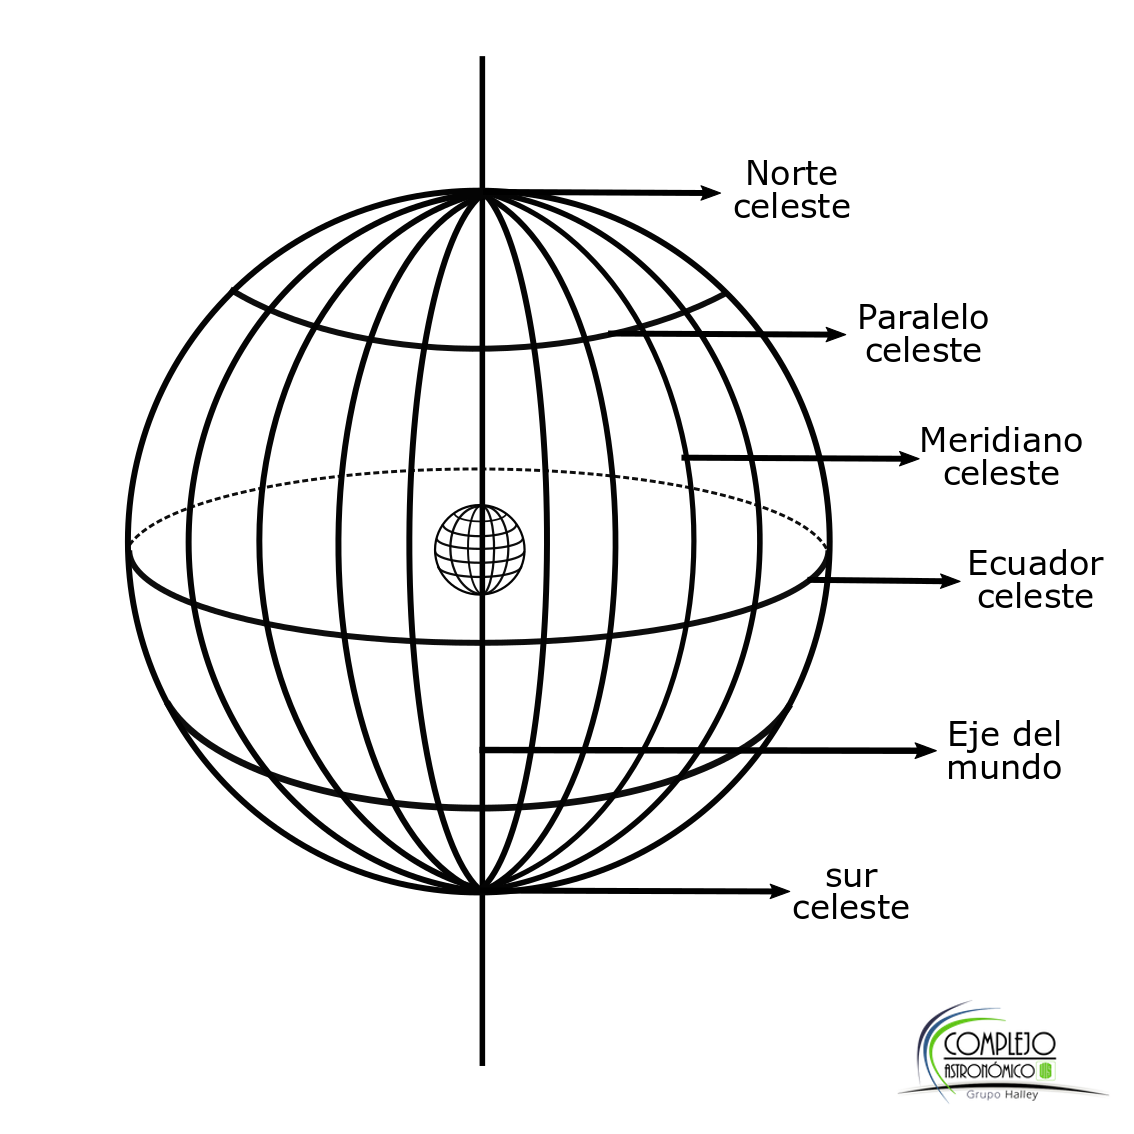
\includegraphics[scale=0.3]{Imagenes/boveda_celeste.png} 
\caption{Bóveda celeste}
\label{b_celeste}
\end{figure}

\section{Planeación de la sesión}
\begin{table}[h!]
\begin{tabular}{|l|l|l|l|}
\hline
\textbf{Etapa}      & \textbf{Tiempo} & \textbf{Actividad}                                        & \textbf{Recursos}                                                           \\ \hline
\textbf{Inicio}     & 30 minutos      & S01AI01                                                   & \begin{tabular}[c]{@{}l@{}}- 20 hojas tamaño carta\\ - Colores\end{tabular} \\ \hline
\textbf{Desarrollo} &                 & \begin{tabular}[c]{@{}l@{}}S01AD01\\ S01AD02\end{tabular} & \begin{tabular}[c]{@{}l@{}}- Proyector\\ - Audio\end{tabular}               \\ \hline
\textbf{Cierre}     &                 & S01AC01                                                   & - Tarjetas                                                                  \\ \hline
\end{tabular}
\end{table}

\subsection{Actividades}
\subsubsection{S01AI01}



\subsubsection{S01AD01}

\subsubsection{S01AD02}

\subsubsection{S01AC01}

\end{document}